\documentclass[11pt,a4paper,notitlepage,twocolumn]{article}

\usepackage[T1]{fontenc}
\usepackage[utf8]{inputenc}
\usepackage[english]{babel}
\usepackage{amsmath}
\usepackage{amsfonts}
\usepackage{amssymb}
\usepackage{verbatim}
\usepackage{listings}
\usepackage{color}
\usepackage{setspace}
\usepackage{epstopdf}
\usepackage{graphicx}
\usepackage{caption}
\usepackage{subcaption}
\usepackage{float}
\usepackage{epstopdf}
\usepackage{hyperref}
\usepackage{dsfont}
\usepackage{braket}
\pagenumbering{arabic}
\usepackage{titling}
\usepackage{fullpage}

\definecolor{codepurple}{rgb}{0.58,0,0.82}
\definecolor{backcolour}{rgb}{0.95,0.95,0.92}
\definecolor{dkgreen}{rgb}{0,0.6,0}
\definecolor{gray}{rgb}{0.5,0.5,0.5}
\definecolor{mauve}{rgb}{0.58,0,0.82}
%\setlength{\parindent}{0pt}

\lstdefinestyle{pystyle}{
  language=Python,
  aboveskip=3mm,
  belowskip=3mm,
  columns=flexible,
  basicstyle={\small\ttfamily},
  backgroundcolor=\color{backcolour},
  commentstyle=\color{dkgreen},
  keywordstyle=\color{magenta},
  numberstyle=\tiny\color{gray},
  stringstyle=\color{codepurple},
  basicstyle=\footnotesize,  
  breakatwhitespace=false
  breaklines=true,
  captionpos=b,
  keepspaces=true,
  numbers=left,
  numbersep=5pt,
  showspaces=false,
  showstringspaces=false,
  showtabs=false,
  tabsize=2
}
\lstdefinestyle{iStyle}{
  language=IDL,
  aboveskip=3mm,
  belowskip=3mm,
  columns=flexible,
  basicstyle={\small\ttfamily},
  backgroundcolor=\color{backcolour},
  commentstyle=\color{dkgreen},
  keywordstyle=\color{magenta},
  numberstyle=\tiny\color{gray},
  stringstyle=\color{codepurple},
  basicstyle=\footnotesize,  
  breakatwhitespace=false
  breaklines=true,
  captionpos=b,
  keepspaces=true,
  numbers=left,
  numbersep=5pt,
  showspaces=false,
  showstringspaces=false,
  showtabs=false,
  tabsize=2
}
\lstdefinestyle{c++style}{
  language=C++,
  keywordstyle=\color{blue}\ttfamily,
  stringstyle=\color{red}\ttfamily,
  commentstyle=\color{green}\ttfamily,
  morecomment=[l][\color{magenta}]{\#}
  aboveskip=3mm,
  belowskip=3mm,
  columns=flexible,
  basicstyle={\small\ttfamily},
  backgroundcolor=\color{backcolour},
  numberstyle=\tiny\color{gray},
  basicstyle=\footnotesize,  
  breakatwhitespace=false
  breaklines=true,
  captionpos=b,
  keepspaces=true,
  numbers=left,
  numbersep=5pt,
  showspaces=false,
  showstringspaces=false,
  showtabs=false,
  tabsize=2
}

\title{\normalsize Fys3150/4150 - Computational Physics\\
\vspace{10mm}
\huge Ising model - Monte Carlo and Metropolis algorithms\\
\vspace{10mm}
\normalsize Due date {\bf Nov $overdue$, 2016}}

% Skriv namnet ditt her og fjern kommenteringa
\author{Magnus Christopher Bareid \\ un: magnucb }

\newcommand{\SE}{Schr\"odinger equation}
\newcommand{\laplacian}{\vec{\nabla}^2}
\newcommand{\eye}{\mathds{I}}
\newcommand\pd[2]{\frac{\partial #1}{\partial #2}}
\def\doubleunderline#1{\underline{\underline{#1}}}

\begin{document}
\noindent
\maketitle
\vspace{5mm}



%\begin{figure}[H]
%	\centering	
%	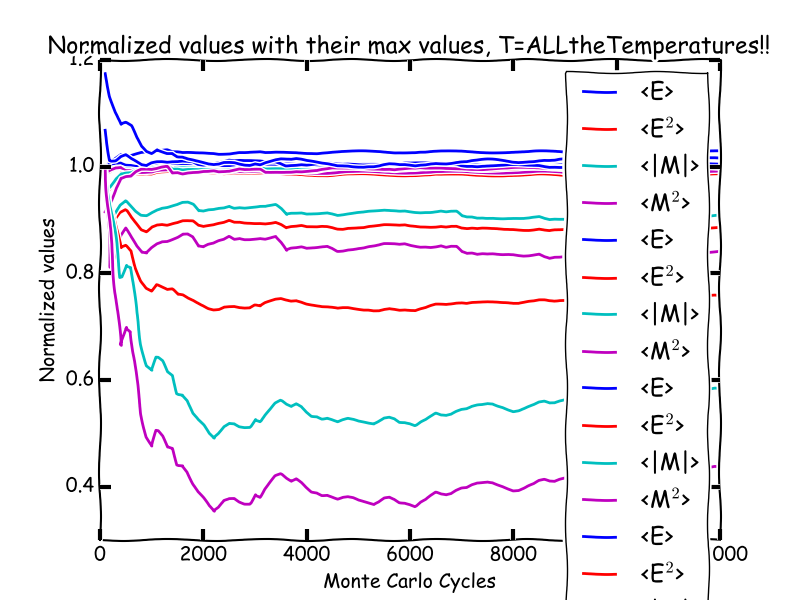
\includegraphics[scale=0.45]{frontpage.png}
%\end{figure}

\begin{abstract}
Empty void %TODO
\end{abstract}



%\begin{center}
%\line(1,0){450}
%\end{center}

\newpage
\tableofcontents

\newpage

\section{Studies of phase transitions in magnetic systems}
\subsection{Introduction}
The aim of this project is to study a widely popular model to simulate phase transitions, the so-called Ising model in two dimensions. At a given critical temperature, this model exhbits a phase transition from a magnetic phase (a system with a finite magnetic moment) to a phase with zero magnetization.

As with all other projects in this course, the important thing is to make the algorithm work. The basic energy calculation of any two-dimensional lattice boils down to this form:
\begin{align}
E = -J \sum^N_{<kl>} s_ks_l
\end{align}
where $s_k$ and $s_l$ are $\pm 1$, $N$ is the total spins in the lattice, $J$ expresses the strength of interaction between neighbouring spins, which are referred to in the summation by $<kl>$ as it sums up interaction only between lattice-neighbours near index $k$ and $l$.

Through the course of this report, we shall investigate different variations on differently-sized lattices and their modelled physical properties.

\subsection{Analytical model of $2\times2$ lattice}





































\end{document}